\let\negmedspace\undefined
\let\negthickspace\undefined
\documentclass[journal]{IEEEtran}
\usepackage[a5paper, margin=10mm, onecolumn]{geometry}
%\usepackage{lmodern} % Ensure lmodern is loaded for pdflatex
\usepackage{tfrupee} % Include tfrupee package

\setlength{\headheight}{1cm} % Set the height of the header box
\setlength{\headsep}{0mm}     % Set the distance between the header box and the top of the text

\usepackage{gvv-book}
\usepackage{gvv}
\usepackage{cite}
\usepackage{amsmath,amssymb,amsfonts,amsthm}
\usepackage{algorithmic}
\usepackage{graphicx}
\usepackage{textcomp}
\usepackage{xcolor}
\usepackage{txfonts}
\usepackage{listings}
\usepackage{enumitem}
\usepackage{mathtools}
\usepackage{gensymb}
\usepackage[breaklinks=true]{hyperref}
\usepackage{tkz-euclide} 
\usepackage{listings}
% \usepackage{gvv}                                        
\def\inputGnumericTable{}                                 
\usepackage[latin1]{inputenc}                                
\usepackage{color}                                            
\usepackage{array}                                            
\usepackage{longtable}                                       
\usepackage{calc}                                             
\usepackage{multirow}                                         
\usepackage{hhline}                                           
\usepackage{ifthen}                                           
\usepackage{lscape}
\usepackage{circuitikz}
\usepackage{comment}
\tikzstyle{block} = [rectangle, draw, fill=blue!20, 
    text width=4em, text centered, rounded corners, minimum height=3em]
\tikzstyle{sum} = [draw, fill=blue!10, circle, minimum size=1cm, node distance=1.5cm]
\tikzstyle{input} = [coordinate]
\tikzstyle{output} = [coordinate]


\begin{document}

\bibliographystyle{IEEEtran}
\vspace{3cm}

\title{12.768}
\author{EE25BTECH11026-Harsha}
 \maketitle
% \newpage
% \bigskip
{\let\newpage\relax\maketitle}

\renewcommand{\thefigure}{\theenumi}
\renewcommand{\thetable}{\theenumi}
\setlength{\intextsep}{10pt} % Space between text and floats


\numberwithin{equation}{enumi}
\numberwithin{figure}{enumi}
\renewcommand{\thetable}{\theenumi}

\textbf{Question}:\\
In the figure, the vectors $\vec{u}$ and $\vec{v}$ are related as $\vec{A}\vec{u}=\vec{v}$ by a transformation matrix $\vec{A}$. The correct choice of $\vec{A}$ is
\begin{figure}[H]
    \centering
    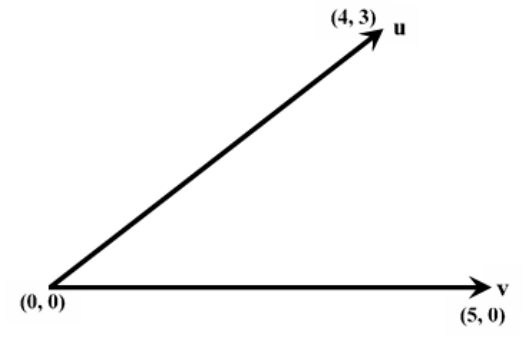
\includegraphics[width=0.4\columnwidth]{figs/Fig-1.png}
    \caption{Figure-1}
    \label{fig:1}
\end{figure}
\begin{enumerate}
\begin{multicols}{4}
    \item $\myvec{\tfrac{4}{5}&&\tfrac{3}{5}\\\tfrac{3}{5}&&-\tfrac{4}{5}}$
    \item $\myvec{\tfrac{4}{5}&&-\tfrac{3}{5}\\\tfrac{3}{5}&&\tfrac{4}{5}}$
    \item $\myvec{\tfrac{4}{5}&&\tfrac{3}{5}\\-\tfrac{3}{5}&&\tfrac{4}{5}}$
    \item $\myvec{\tfrac{4}{5}&&-\tfrac{3}{5}\\\tfrac{3}{5}&&-\tfrac{4}{5}}$
\end{multicols}
\end{enumerate}

\solution \\
Let us solve the given question theoretically and then verify the solution computationally.\\
\\
Given,
\begin{align}
    \vec{u}=\myvec{4\\3} \qquad \vec{v}=\myvec{5\\0}
\end{align}
From ~\ref{fig:1},
\begin{align}
    \|\vec{u}\|=\|\vec{v}\|=5 \; units
\end{align}
This implies, $\vec{A}$ is a rotation matrix.\\
Rotation matrix $\vec{A}$ is given by 
\begin{align}
    \vec{A}=\myvec{\cos{\theta}&&-\sin{\theta}\\\sin{\theta}&&\cos{\theta}}
\end{align}
where $\theta$ is the angle between the vectors in counter-clockwise sense.\\
\begin{align}
    \therefore \myvec{\cos{\theta}&&-\sin{\theta}\\\sin{\theta}&&\cos{\theta}}\myvec{4\\3}=\myvec{5\\0}
\end{align}
\newpage
\vspace*{0.25cm}
\begin{align}
    \myvec{4\cos{\theta}-3\sin{\theta}\\4\sin{\theta}+3\cos{\theta}}=\myvec{5\\0}
\end{align}
The above equation can be re-arranged as,
\begin{align}
    \myvec{4&&-3\\3&&4}\myvec{\cos{\theta}\\\sin{\theta}}=\myvec{5\\0} \label{eq:1}
\end{align}
We need to solve for $\cos{\theta}$ and $\sin{\theta}$ to get the transformation matrix $\vec{A}$.\\
\\
We can see that in ~\eqref{eq:1}, the columns of the coefficient matrix are orthogonal to each other and also the column vectors have the same norm.
\begin{align}
    \therefore \frac{1}{5}\myvec{4&&-3\\3&&4}\myvec{\cos{\theta}\\\sin{\theta}}=\frac{1}{5}\myvec{5\\0}
\end{align}
\begin{align}
    \implies \myvec{\tfrac{4}{5}&&-\tfrac{3}{5}\\\tfrac{3}{5}&&\tfrac{4}{5}}\myvec{\cos{\theta}\\\sin{\theta}}=\myvec{1\\0}
    \label{eq:2}
\end{align}
In equation ~\eqref{eq:2}, the coefficient matrix is an orthogonal matrix.
\begin{align}
    \implies \vec{A}\vec{x}=\vec{b} 
    \Rightarrow 
    \vec{A}^{\top}\vec{A}\vec{x}=\vec{A}^{\top}\vec{b}
    \Rightarrow
    \vec{x}=\vec{A}^{\top}\vec{b} \qquad \brak{\because \vec{A}^{\top}\vec{A}=\vec{I}}
\end{align}
\begin{align}
    \therefore \myvec{\cos{\theta}\\\sin{\theta}}=\myvec{\tfrac{4}{5}&&\tfrac{3}{5}\\-\tfrac{3}{5}&&\tfrac{4}{5}}\myvec{1\\0}
\end{align}
\begin{align}
    \therefore \myvec{\cos{\theta}\\\sin{\theta}}=\myvec{\tfrac{4}{5}\\-\tfrac{3}{5}}
\end{align}
\begin{align}
    \implies \vec{A}=\myvec{\tfrac{4}{5}&&\tfrac{3}{5}\\-\tfrac{3}{5}&&\tfrac{4}{5}}
\end{align}


\end{document}
